\documentclass{article}
\usepackage{amsmath,amssymb}
\usepackage{fullpage}
\usepackage{mathrsfs}
\usepackage{setspace}
\usepackage{graphicx}
\usepackage{listings}
\renewcommand{\baselinestretch}{1.3}
\pagestyle{empty}
\usepackage{color}
\definecolor{dkgreen}{rgb}{0,0.6,0}
\definecolor{gray}{rgb}{0.5,0.5,0.5}
\definecolor{mauve}{rgb}{0.58,0,0.82}

\lstset{frame=tb,
	language=Matlab,
	aboveskip=3mm,
	belowskip=3mm,
	showstringspaces=false,
	columns=flexible,
	basicstyle={\small\ttfamily},
	numbers=none,
	numberstyle=\tiny\color{gray},
	keywordstyle=\color{blue},
	commentstyle=\color{dkgreen},
	stringstyle=\color{mauve},
	breaklines=true,
	breakatwhitespace=true,
	tabsize=4
}
\begin{document}
\noindent{\bf Homework 2}

\noindent{\bf Jingmin Sun}

\noindent{\bf 661849071}

\begin{enumerate}
\item 

We can observe that around $x=1$, the function touches $x$ axis, but not cross it, so we cannot use bisection method to find this root directly. Instead of that, we can find the local minimum of the function, and the local minimum will be the one that touches $x$ axis. To find the minimum, we can differentiate the function since it's a nice smooth function. If the derivative equals 0 at some point, then it will be the local minimum $\bar{x}$, and we can find the value of $f(\bar{x})$, if it is positive, then the original graph does not have solution around $x=1$, and if it is zero, then we get the answer, and if it is negative, we can use bisection method directly to the original function.

So, our goal now is find the root for the derivative of the original function by bisection method, and the derivative of the original function is $5x^4-4x^3-1$, and we can observe that it cross the x-axis around 1, so we can apply bisection method to find the root for it around 1.

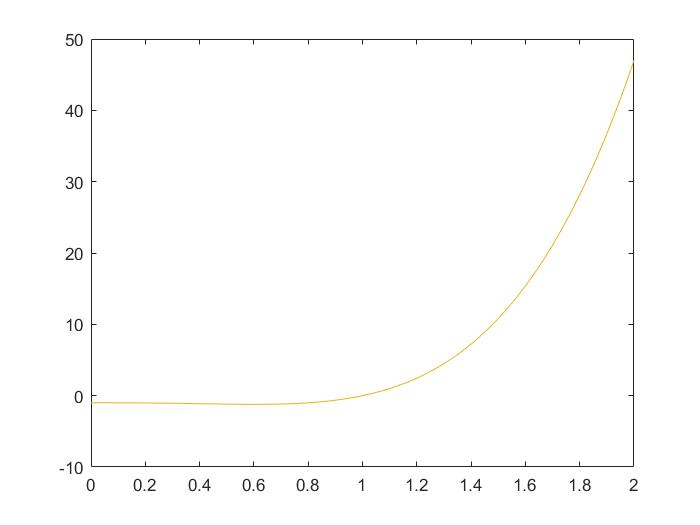
\includegraphics[width=7cm]{1.jpg}

\item
\begin{enumerate}
\item
To compute the square root of a positive constant $\alpha$, it's same to solve the equation $x = \sqrt{\alpha}$, since we can only involve $+,-,*,/$, so we can choose to find the root of\[f(x) = x^2 -\alpha\] 
\item
When $\alpha =3$, we need to find the root for $f(x) = x^2-3$,  suppose $[a_0,b_0] = [1,2]$, since \begin{align*}
f(a_0) &= f(1) = 1-3 =-2\\
f(b_0) &= f(2) = 4 -3 =1\\
\therefore f(a_0)f(b_0) &= -2\cdot 1 =-2 <0
\end{align*}
the choice of $[a_0,b_0]$ is valid.
Let $c_0 = \dfrac{a_0+b_0}{2} = \dfrac{3}{2}$, and\begin{align*}
f(c_0) &= f\left(\frac{3}{2}\right) = \frac{9}{4} -3 = -\frac{3}{4}\\
\because f(a_0)f(c_0) &= -2 \cdot -\frac{3}{4} = \frac{3}{2}>0\\
f(b_0)f(c_0) &= 1 \cdot -\frac{3}{4} = -\frac{3}{4} <0\\
\therefore [a_1,b_1] &= [c_0, b_0] = \left[\frac{3}{2}, 2\right]\\
c_1&=\frac{a_1+b_1}{2} = \frac{\frac{3}{2}+2}{2} =\frac{7}{4}
\end{align*}

\item
The update formula for Newton's method is \begin{align*}
x_{j+1}&= x_j-\dfrac{f(x_j)}{f'(x_j)}\\
&=x_j -\dfrac{x_j^2-3}{2x_j}
& \forall j = 1,2,3\cdots
\end{align*}
Choose $x_0 = \frac{3}{2}$, since $f(x_0)= -\frac{3}{4}$, which is near zero, so it's a good choice.
\begin{align*}
x_{1}&=x_0 -\dfrac{x_0^2-3}{2x_0}\\
&=x_0-\dfrac{x_0}{2}+\dfrac{3}{2x_0}\\
&=\dfrac{x_0}{2}+\dfrac{3}{2x_0}\\
&=\dfrac{\frac{3}{2}}{2}+\dfrac{3}{2\frac{3}{2}}\\
&=\frac{7}{4}\\
x_{2}&=x_1 -\dfrac{x_1^2-3}{2x_1}\\
&=x_1-\dfrac{x_1}{2}+\dfrac{3}{2x_1}\\
&=\dfrac{x_1}{2}+\dfrac{3}{2x_1}\\
&=\dfrac{\frac{7}{4}}{2}+\dfrac{3}{2\frac{7}{4}}\\
&=\frac{97}{56}\\
\end{align*}
\end{enumerate}
\item
\begin{enumerate}
\item
Sketch:

~\\


~\\


~\\


~\\


Since the solution for $y+t = e^{-y}$ has exactly the same solution as $y+t - e^{-y} =0$, let $f(y) = y+t - e^{-y}$, and $f'(y) =1+ e^{-y} >0$ follows, so $f(y)$ is a monotony increasing function, which means it has only one intersection to the $f(y) = 0$, so, no matter what $t$ is, there is only one solution.
\item
The updated formula for secant method is\begin{align*}
y_{j+1}&= y_j - \dfrac{f(y_j)(y_j-y_{j-1})}{f(y_j)-f(y_{j-1})}\\
&= y_j - \dfrac{(y_j+t - e^{-y_j})(y_j-y_{j-1})}{(y_j+t - e^{-y_j})-(y_{j-1}+t - e^{-y_{j-1}})}\\
&= y_j - \dfrac{(y_j+t - e^{-y_j})(y_j-y_{j-1})}{(y_j-y_{j-1}) +( e^{-y_{j-1}}-e^{-y_j})}\\
\end{align*}
\end{enumerate}
\item
To find the root for $\cos(x) =2\sin(x)$, it's same to compute the root for $f(x) = \cos(x) -2\sin(x)$.  Since we aim to find the smallest positive root, we can draw the graph first,
\begin{center}
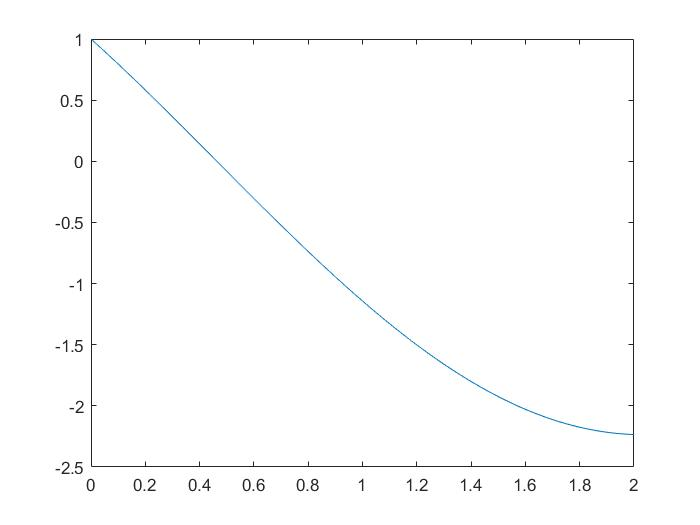
\includegraphics[width=5cm]{4.jpg}
\end{center}

 and we can observe that the smallest positive root lies between 0 and 1, which means we can set the initial interval to $[0,1]$, and for stopping criterion, we need to make the computational root to lies in the $10^{-6}$ neighborhood of $\bar{x}$, so we need the interval of final iteration no larger than $ 10^{-6}$, so the stopping criterion is $\dfrac{b-a}{2} \leq 0.5 \cdot 10^{-6}$

\lstinputlisting[language=Matlab, numbers=left, stepnumber=1, firstline=1,caption={bisection.m function},frame=single]{bisection.m}
\lstinputlisting[language=Matlab,caption={output}]{forth.txt}

\item

My initial guess is $x_0=1$, and there are three stopping criteria in my algorithm: \begin{itemize}
\item
If the difference between two iteration is relatively small, then we stop
\item
If we have large amount iteration, we stop.
\item
Since we wanna find the solution that lies between 1 and 3, so if $x>3$, then we stop
\end{itemize}

\lstinputlisting[language=Matlab, numbers=left, stepnumber=1, firstline=1,caption={newton.m function},frame=single]{newton.m}
\lstinputlisting[language=Matlab,caption={output}]{fifth.txt}

\item
\begin{enumerate}
\item
First, let's compute the derivatives of $f$
\begin{align*}
f'(x)&=\dfrac{d x^2\sin x^2}{d x}\\
&=2x\sin x^2+2x^3\cos x^2\\
f'(0)&=0\\
f''(x) &=\dfrac{d 2x\sin x^2+2x^3\cos x^2}{d x}\\
&=2\sin x^2+4x^2\cos x^2+6x^2\cos x^2-4x^4\sin x^2\\
&=2\sin x^2+10x^2\cos x^2-4x^4\sin x^2\\
f''(0) &=0\\
f'''(x)&= \dfrac{d 2\sin x^2+10x^2\cos x^2-4x^4\sin x^2}{d x}\\
&=4x\cos x^2+20x\cos x^2-20x^3\sin x^2-16x^3\sin x^2-8x^4\cos x^2\\
&=4x\cos x^2+20x\cos x^2-36x^3\sin x^2-8x^4\cos x^2\\
f'''(0) &=0\\
f^{(4)}(x)&= \dfrac{d 4x\cos x^2+20x\cos x^2-36x^3\sin x^2-8x^4\cos x^2}{d x}\\
&=4\cos x^2+8x^2\sin x^2+20\cos x^2-40x^2\sin x^2-108x^2\sin x^2-72x^4\cos x^2-32x^3\cos x^2 + 16x^4\sin x^2\\
f^{(4)}(0)&=24
\end{align*}
Thus, the multiplicity of the root is $4$.
\item
The backward error is \begin{align*}
|f(x_a)| &= |(0.01)^2\sin (0.01^2)|\\
&=9.9999999983\times 10^{-9}\\
\end{align*}

And the forward error is \begin{align*}
|r-x_a|&= |0-0.01|\\&= 0.01	
\end{align*}
\end{enumerate}

\item
We can calculate the derivative for the function first, which is \begin{align*}
f'(x) &= (x-2)(x-3)(x-4)+(x-1)(x-3)(x-4)+(x-1)(x-3)(x-4)+(x-1)(x-2)(x-3)\\
f'(4) &= (x-1)(x-2)(x-3)\\
&= 3\cdot 2\cdot 1\\
&=6
\end{align*}
And we can get \begin{align*}
\Delta x &= -\dfrac{h(x)}{f'(x)}\epsilon\\
&=-\dfrac{-4^6}{6}\epsilon\\
&=\frac{2048}{3}\epsilon\\
&\approx 682.67 \epsilon\\
\mbox{When }& \epsilon =10^{-6}\\
\Delta x &=6.8267\times 10^{-4}\\
\hat{x} &= 4+6.8267\times 10^{-4}\\
\mbox{When }& \epsilon =10^{-8}\\
\Delta x &=6.8267\times 10^{-6}\\
\hat{x} &= 4+6.8267\times 10^{-6}\\
\end{align*}

And we can observe the answer calculated by MATLAB:
\lstinputlisting[language=Matlab,caption={output}]{seventh.txt}
\end{enumerate}

\end{document}